
\chapter{Anhang}
\section{Über das Statistik-Modul des AMIDAR-Debuggers ermittelte Leistungsdaten}

\subsection{Echo-Server über 10 Verbindungen}
\begin{tabular}{lc}
jumpBytecodes & 16842753\\
total & 545259268 \\
distributedToken & 2004025412 \\
axi.transaction& 1\\
cache.hit & 65793\\
cache.hitrate& 0.996109\\
cache.miss& 257\\
outputFifoEmptyAtferFirstTransaction&16780707
\end{tabular}
\subsection{Senden von Daten über eine Verbindung}

\begin{tabular}{lc}
jumpBytecodes & 537919489\\
total & 545259268 \\
distributedToken & 393412689 \\
axi.transaction& 1\\
cache.hit & 65793\\
cache.hitrate& 0.9960939\\
cache.miss& 258\\
outputFifoEmptyAtferFirstTransaction & 16781085
\end{tabular}

\section{Wireshark Screenshots}
\begin{figure}
	\centering
	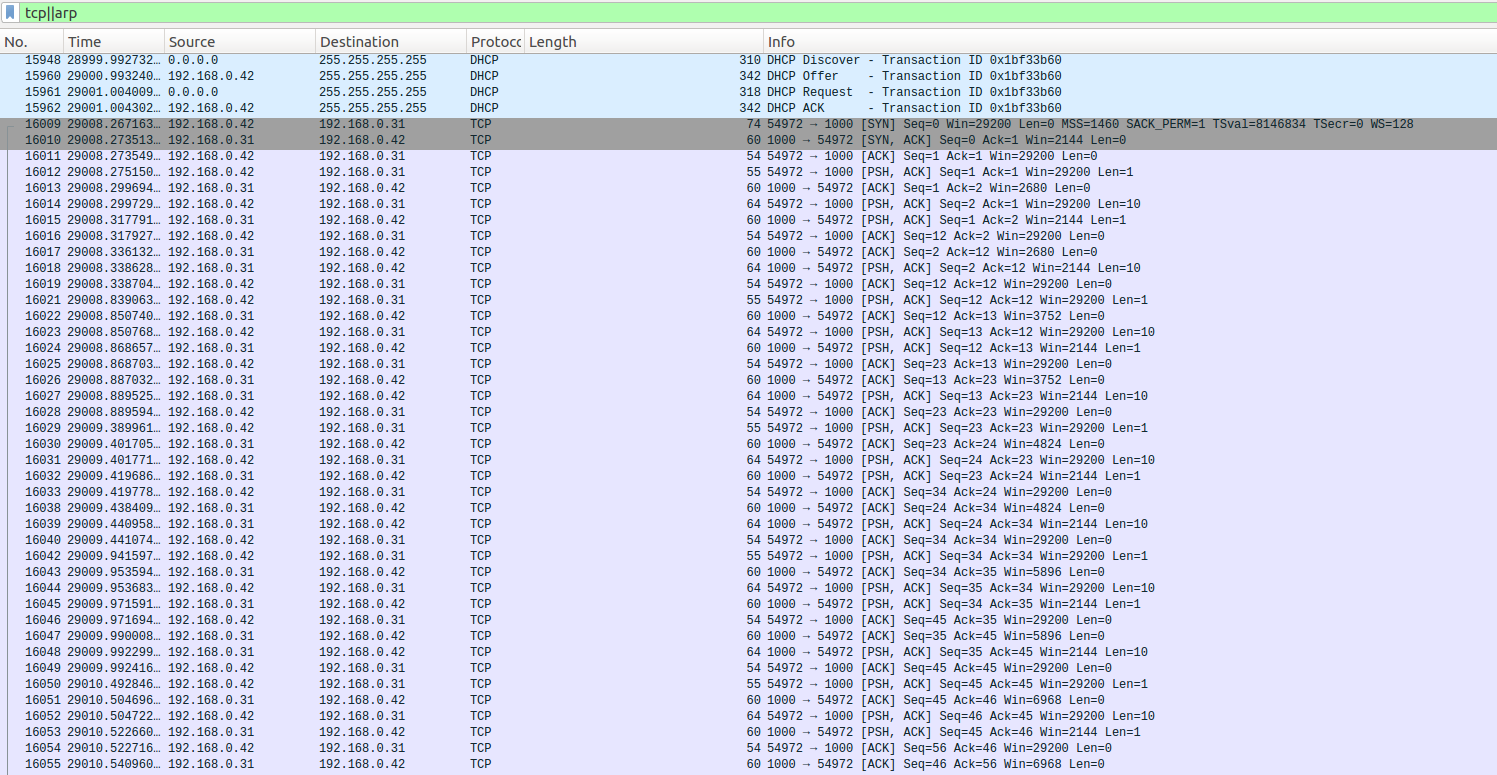
\includegraphics[width=1\textwidth]{Graphics/dhcpHD.png}
	\caption{DHCP, Drei-Wege-Handschlag, Datenübertragung}
\end{figure}

\begin{figure}[h]
	\centering
	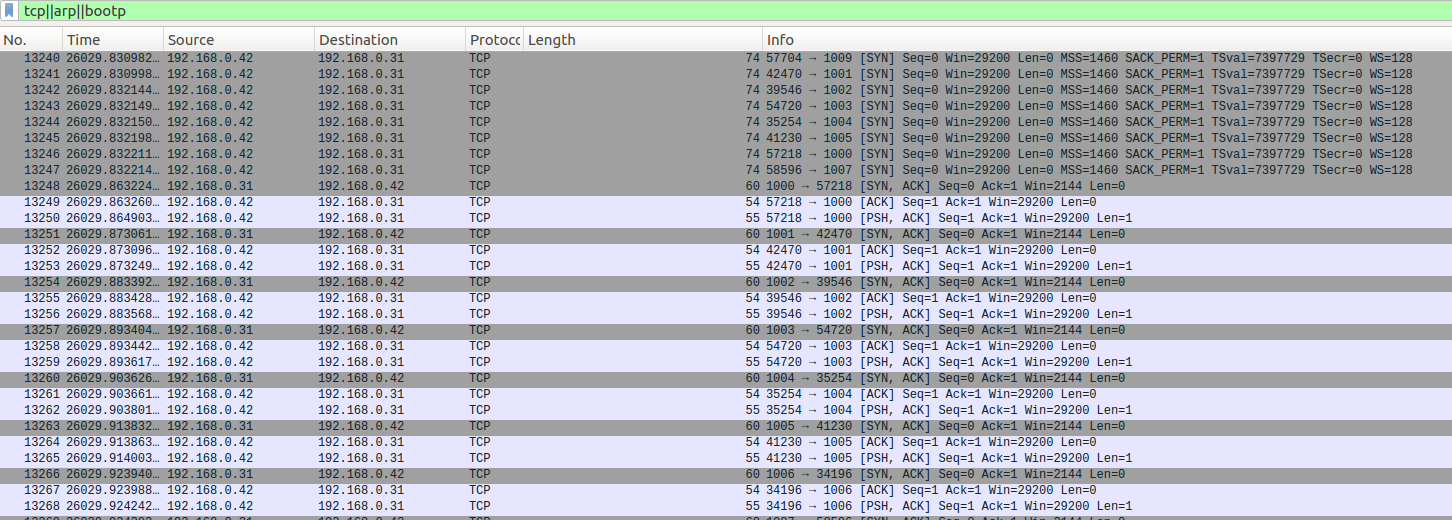
\includegraphics[width=1\textwidth]{Graphics/MTCon.png}
	\caption{Gleichzeitiger Verbindungsaufbau mehrerer Verbindungen}
\end{figure}

\begin{figure}[h]
	\centering
	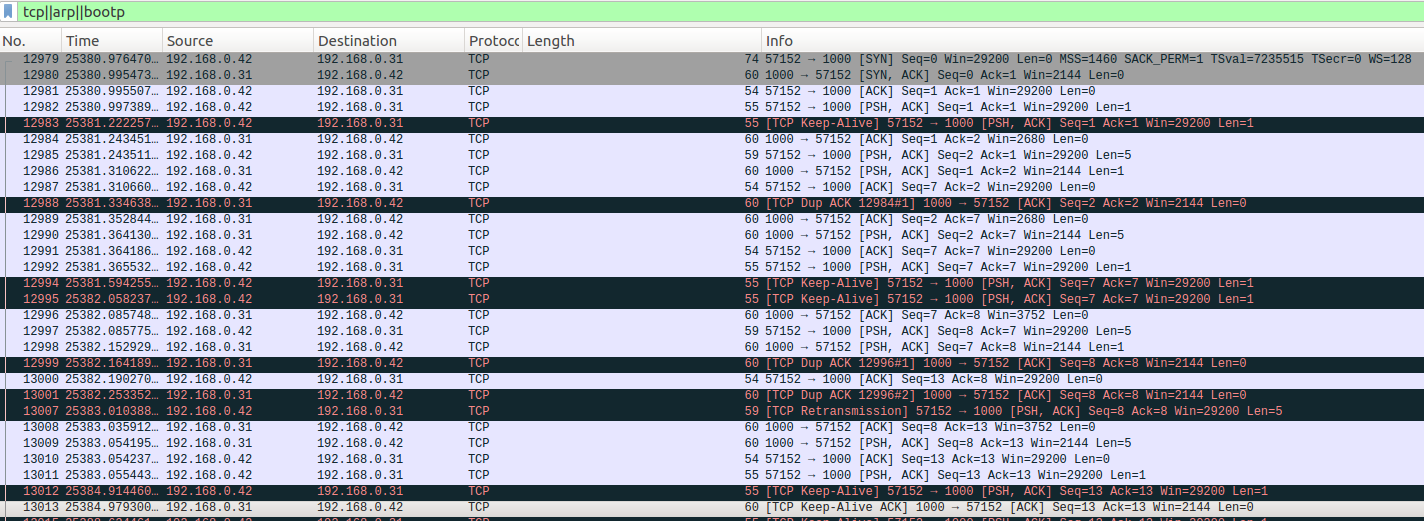
\includegraphics[width=1\textwidth]{Graphics/latency.png}
	\caption{keep-alive und Retransmissions, wegen schwankender Latenz, bei großen Datenpaketen}
\end{figure}